\documentclass[chaptersright]{informeutn}
\usepackage{circuitikz}

% Datos del informe
\materia{Electronica Aplicada I}
\titulo{Trabajo Práctico 2}
\comision{3R2}
\autores{
          Gaston Grasso - 401892\\
          Franco Palombo - 401910\\
          Angelo Prieto - 401012}
\fecha{21/05/2025}

\begin{document}
  \maketitle

  \tableofcontents
  \setcounter{page}{1}
  \thispagestyle{plain}

  \chapter{Introducción} 

    En el marco de la asignatura \textit{Electrónica Aplicada I}, se llevó a cabo un trabajo práctico centrado en la
    construcción y análisis de una fuente de alimentación de tensión variable. Este tipo de fuente resulta fundamental
    en entornos de laboratorio y desarrollo electrónico, ya que permite alimentar circuitos con distintos
    requerimientos de tensión de forma estable y segura.

    El diseño de la fuente fue provisto por el docente a cargo, por lo que el enfoque del trabajo no estuvo en la etapa
    de diseño conceptual, sino en la interpretación, armado y validación funcional del circuito.

    La realización del proyecto se desarrolló de manera progresiva, abordando dos etapas principales de la
    fuente, primero: fuente no regulada y luego, fuente regulada. Esta metodología permitió realizar ensayos parciales,
    facilitando la comprensión del comportamiento eléctrico en cada etapa.

    El circuito final tiene la capacidad de entregar una tensión de salida variable entre 0 y 30\,V con una corriente
    máxima de 1.5\,A. Se efectuaron ensayos destinados a verificar su desempeño, incluyendo mediciones de
    \textit{ripple}, control de regulación de voltaje, y análisis de temperatura en el regulador LM317. Más allá de su
    valor académico, la fuente construida será utilizada como herramienta de alimentación en futuros trabajos
    prácticos, reafirmando así su utilidad práctica y formativa.

  \chapter{Planeamiento e introduccion teorica}
    Para la realizacion del trabajo practico, es necesario tener un conocimiento basico de los elementos, etapas y
    procedimientos los cuales se ven involucrados. Entre ellos estan:
    \begin{itemize}
      \item Transformador.
      \item Rectificacion.
      \item Filtrado.
      \item Regulacion.
      \item Otros.
    \end{itemize}

      \section{Transformador}
        El transformador cumple dos funciones principales:
        \begin{itemize}
          \item Proporciona aislamiento galvanico entre la red de 220 V y la fuente mediante acoplamiento magnetico.
          \item Reduce la tension de 220 V a un valor determinado por la relacion entre el bobinado de entrada y el 
            boninado de salida, acorde a las necesidades de lo que se busca alimentar.
        \end{itemize}

        Para este trabajo practico, se emplea un transformador de $12+12V$. Esto significa que el transformador tiene
        dos cables de entrada, y tres de salida. De los tres cables, dependiendo de cual se tome como referencia, el
        transformador puede utilizarse como una fuente con salida positiva y negativa, donde por un lado hay $+12V$ y
        por el otro $-12V$, o como una fuente con dos diferentes salidas de voltaje, del mismo signo, teniendo $+12V$ o
        $+24V$. Para el trabajo practico, se utilizo el transformador como fuente $+12V/+24V$. Para ello, se conecto
        uno de los terminales de la punta del bobinado secundario como referencia, y con un interruptor SPDT
        (\textit{Singe-Pole Doble-Throw}), es posible seleccionar si se usa el 'punto alto' o el 'punto bajo' del
        transformador.

        \begin{figure}[!h]
          \noindent
          \centering
          \begin{circuitikz}[american]
            \draw (0,0) to [sV, l=$220V$] ++(0,2) -- ++(1,0)
            node[transformer core, circuitikz/inductors/coils=6,
            anchor=A1](T){};
            \draw (T.A2) -| (0,0);
            \draw (T-L2.midtap) to[short, *-] (T.B1 |- T-L2.midtap);
            \draw (T.B2) to[short, -o] ++(1.2,0);
            \draw (T.B1) ++(0.6,-0.55) node[spdt, rotate=180](SW){} ;
            \draw (T.B1) -| (SW.out 2);
            \draw (T-L2.midtap) -| (SW.out 1);
            \node [ocirc] at (SW.in){};
            \draw (T.B2) ++(1.2,0) to[open, v_<=$12/24V$] (SW.in);
          \end{circuitikz}
          \caption{Esquema del transformador y el selector de punto.}
        \end{figure}


      \section{Rectificacion}
        La salida de voltaje del transformador sigue siendo una onda sinusoidal con la misma frecuencia que la linea,
        por lo que para poder usarla es necesario eliminar el semiciclo negativo. Para ello, podemos emplear un
        conjunto de diodos configurados como rectificador de onda completa.

        La función del rectificador de onda completa es convertir la tensión alterna en una pulsante, con solo
        semiciclos positivos y sin pedrida de los semiciclos negativos, como si pasa en un rectificador de media
        onda.
        \begin{figure}[!h]
          \noindent
          \centering
          \begin{minipage}[t][5cm][c]{0.4\textwidth}
            \centering
            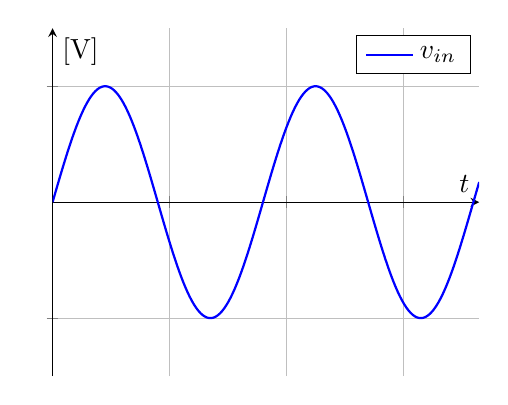
\begin{tikzpicture}
              \begin{axis}[
                  axis lines=middle,
                  xlabel={$t$},
                  ylabel={[V]},
                  xticklabels={},
                  yticklabels={},
                  domain=0:730,
                  samples=200,
                  grid=both,
                  width=7cm,
                  height=6cm,
                  ymin=-3, ymax=3,
                  xmin=0, xmax=730,
                ]
                \addplot[blue, thick] {2*sin(x)};
                \addlegendentry{$v_{in}$}
              \end{axis}
            \end{tikzpicture}
          \end{minipage}
          \begin{minipage}[t][5cm][c]{0.4\textwidth}
            \centering
            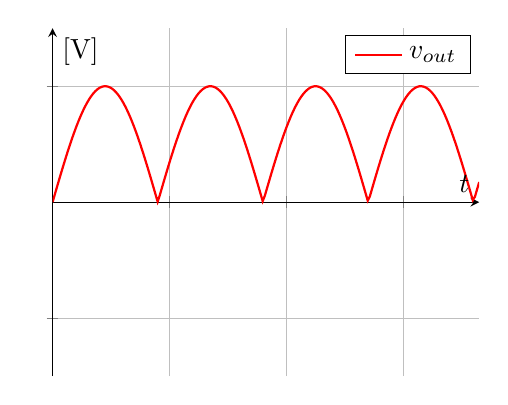
\begin{tikzpicture}
              \begin{axis}[
                  axis lines=middle,
                  xlabel={$t$},
                  xticklabels={},
                  yticklabels={},
                  ylabel={[V]},
                  domain=0:730,
                  samples=200,
                  grid=both,
                  width=7cm,
                  height=6cm,
                  ymin=-3, ymax=3,
                  xmin=0, xmax=730,
                ]
                \addplot[red, thick] {abs(2*sin(x))};
                \addlegendentry{$v_{out}$}
              \end{axis}
            \end{tikzpicture}
          \end{minipage}
          \caption{Señales de entrada y salida}
        \end{figure}

        La ventaja del rectificador de onda completa es que permite aprovechar la totalidad de la corriente
        alterna. El circuito que cumple esa función se lo conoce como puente de diodos. Un detalle a tener en cuenta,
        es que debido a que el rectificador de onda completa convierte el semiciclo negativo en uno positivo, el
        periodo en el cual la señal se repite disminuye, por lo tanto, si la entrada es una onda senoidal de 50$\Hz$,
        a la salida obtenemos una señal pulsante con el doble de la frecuencia, en este caso, 100$\Hz$.
        \begin{figure}[H]
          \noindent
          \centering
          \begin{minipage}[t][8cm][c]{0.4\textwidth}
            \centering
            \begin{circuitikz} [circuitikz/diodes/scale=0.7, american]
              \draw (0,0) coordinate(top bridge) to [full diode, *-*, l={\footnotesize D2}, f={i}] ++(2,-2) coordinate(right bridge)
              to [full diode, *-*, invert, l={\footnotesize D4}] ++(-2,-2) coordinate (bottom bridge)
              to [full diode, *-*, invert, l={\footnotesize D3}, f_<=i ] ++(-2,2) coordinate (left bridge)
              to [full diode, *-*, l={\footnotesize D1}] (0,0);
        
              \draw (top bridge) to[short, -o, f_<={i},] ++(-3.5,0) coordinate(inA);
              \draw (bottom bridge) to[short, -o, f=i] ++(-3.5,0) coordinate(inB);
              \draw (right bridge) to[short] ++(1,0) coordinate(outA);
              \draw (left bridge)to[short] ++(-0.3,0) to[short] ++(0,-3) to[short, f_<=i] ++(5.3,0) coordinate(outB);
        
              \draw (outA) to[R, v_=$v_L$, f=i] (outB);
        
              \node at ($(inA)!0.5!(inB)$) []{$v_{in}$};
        
              \node at ($(inA) +(-0.4,0)$) []{+};
              \node at ($(inB) +(-0.4,0)$) []{-};
        
            \end{circuitikz}
            \caption{Semiciclo positivo}
          \end{minipage}
          \hspace{1cm}
          \begin{minipage}[t][8cm][c]{0.4\textwidth}
            \centering
            \begin{circuitikz} [circuitikz/diodes/scale=0.7, american]
              \draw (0,0) coordinate(top bridge) to [full diode, *-*, l={\footnotesize D2}] ++(2,-2) coordinate(right bridge)
              to [full diode, *-*, invert, l={\footnotesize D4}, f<={i}] ++(-2,-2) coordinate (bottom bridge)
              to [full diode, *-*, invert, l={\footnotesize D3}] ++(-2,2) coordinate (left bridge)
              to [full diode, *-*, l={\footnotesize D1}, f>_={i}] (0,0);
        
              \draw (top bridge) to[short, -o, f_=i] ++(-3.5,0) coordinate(inA);
              \draw (bottom bridge) to[short, -o, f<=i] ++(-3.5,0) coordinate(inB);
              \draw (right bridge) to[short] ++(1,0) coordinate(outA);
              \draw (left bridge)to[short] ++(-0.3,0) to[short] ++(0,-3) to[short, f_<=i] ++(5.3,0) coordinate(outB);
        
              \draw (outA) to[R, v_=$v_L$, f = i] (outB);
        
              \node at ($(inA)!0.5!(inB)$) []{$v_{in}$};
        
              \node at ($(inA) +(-0.4,0)$) []{-};
              \node at ($(inB) +(-0.4,0)$) []{+};
        
            \end{circuitikz}
            \caption{Semiciclo negativo}
          \end{minipage}
        \end{figure}


        \subsection{Eleccion de diodos}
          Es importante saber que el diodo tiene limites de operacion. En estos limites se dictan las capacidades
          maximas de operacion del diodo, por ejemplo: Corriente en directa maxima, Voltaje de ruptura en directa,
          Voltaje de ruptura en inversa, etc. Segun los requerimientos de la fuente y las condiciones de trabajo de los
          diodos, podemos determinar cual diodo utilizar.

          La corriente maxima continua que va a necesitar la fuente, esta determinada por la hoja de datos del LM317,
          el elemento regulador que pone la primera limitacion a la salida de corriente. En la hoja de datos, se
          especifica que la entrega maxima de corriente del LM317 es de $1.5\A$, pero, por cortos periodos de tiempo,
          puede entregar hasta $2.1\A$.

          Teniendo en cuenta lo anterior mencionado, y sabiendo que por cada rama del puente de diodos pasa la mitad de
          la corriente total, podemos determinar que, como maximo, por cada diodo va a pasar $1.05\A$, superando el
          maximo de la serie 1N400X (1-7). Debido a esto, elegimos diodos de 3A de la serie 1N540X (1-8) ya que diodos
          de $2\A$ no se fabrican.

          Un dato no menor es el de los voltajes maximos en directa y en inversa. Debido a que el potencial mas alto
          que va a ver la fuente es el de la salida del transformador, podemos determinar el voltaje maximo en directa
          e inversa que van a experimentar los diodos durante su ciclo de trabajo utilizando:
          \begin{equation}
            V_p = V_{EF} \cdot \sqrt{2}
            \label{voltaje.pico}
          \end{equation}

          Utilizando (\ref{voltaje.pico}) y sabiendo que el transformador puede entregar como maximo $24VAC$, la
          tension pico es:
          \begin{equation*}
            V_p = 24V \cdot \sqrt{2} = 33.94V
          \end{equation*}

          Segun la hoja de datos, el 1N5400 es un buen candidato. Incluso si quisesemos tener mas seguridad, se podria
          usar el 1N5401, que tiene hasta $100\V$ de voltaje de polarizacion en inversa ($V_{RRM}$). A pesar de ello,
          en el kit de la fuente vinieron 4 diodos 1N5408.


      \section{Filtrado}
        Despues de que la entrada de alimentacion pasa por el rectificador de onda completa, la señal con la que se
        trabaja es una senoidal pulsante de $100\Hz$. A pesar de que ya no tiene semiciclos negativos, el hecho de que
        siga siendo una señal pulsada no es deseable. Para ello, se emplean una serie de filtros que permiten eliminar
        el aspecto pulsante de la entrada de alimentacion y convertirla en una señal realmente continua. Para lograr
        ese cambio en la señal se usan conjuntos capacitores que funcionan como almacenadores de energia durante el
        flanco de subida de la señal pulsante, y durante el flanco de bajada funcionan como fuentes que compensan
        la caida de la señal pulsante. Dependiendo del voltaje y la carga a la que se planea someter la fuente, se
        puede calcular que capacitor es necesario para la fuente:
        \begin{equation}
            C = \frac{I_{L}}{2 \cdot f_{salida} \cdot \varDelta V}
        \end{equation}

        Sabiendo que la corriente maxima que puede llegar a requerir la fuente es de $2\A$, la diferencia de voltaje
        es aproximadamente $34\V$ y la frecuencia $100\Hz$:
        \begin{equation*}
          C = \frac{2\A}{2 \cdot 100\Hz \cdot 34\V}
        \end{equation*}

      \section{Regulación}
        Aunque ya tengamos nuestra señal rectificada y filtrada, es necesario incluir en nuestra fuente algun
        dispositivo que se encargue de que, con las fluctuaciones de corriente debido a las distintas cargas, hacer que
        la tension permanezca constante. Para ello se utiliza un regulador lineal, en este caso, ajustable como es el
        LM317. El regulador, ademas de mantener una salida de tension constante, reduce el ripple de la señal en el
        orden de unas 1000 veces.

        \subsection{Especificaciones y calculos}
          El LM317, se comercializa en diferentes formatos, con los cuales varian el factor de forma y la potencia
          disipada. Los mas comunes son el TO-220 y el TO-3, cuyos encapsulados disipan $15\W$ y $20\W$ respectivamente.
          \begin{figure}[H]
            \centering
            \begin{minipage}[b]{0.3\textwidth}
                \centering
                \includegraphics[width=\textwidth]{pictures/to220.jpg}
                \caption*{TO-220}
            \end{minipage}
            \hspace{1cm}
            \begin{minipage}[b]{0.3\textwidth}
                \centering
                \includegraphics[width=\textwidth]{pictures/to3.jpg}
                \caption*{TO-3}
            \end{minipage}
          \end{figure}
          En nuestro caso, empleamos el formato TO-220.
          \begin{center}
            \begin{minipage}{0.45\textwidth}
              \centering
              \includegraphics[width=\linewidth]{pictures/Salida_lm317.png}
            \end{minipage}
            \hfill
            \begin{minipage}{0.5\textwidth}
              Por otro lado, el regulador cuenta con 3 terminales: INPUT, OUTPUT y ADJ. Entre OUTPUT y ADJ se establece
              una tensión constante $V_{REF} = 1.25\,\mathrm{V}$. Además, $I_{ADJ} = 50\,\mu\mathrm{A}$ \quad y \quad
              $I_1 = I_{REF} = \dfrac{V_{REF}}{R_1}$.
            \end{minipage}
            \vspace{5mm}
          \end{center}

        En cuanto a los limites de operacion:

        \begin{center}
          $I_{MAX}=1.5\A \qquad V_{Diff-MAX}=V_{in}-V_{out}=40\V \qquad T_{juntura-max}=125\Celsius$
        \end{center}

        Ahora para el calculo de la tension de salida:

        \begin{align*}
          V_{OUT} &= I_1 \times R_1 + \left(I_1 + I_{ADJ}\right) \times R_2
          = I_1 \times R_1 + I_1 \times R_2 + I_{ADJ} \times R_2 \\[6pt]
          V_{OUT} &= I_1 (R_1 + R_2) + I_{ADJ} \times R_2
          = \frac{1.25}{R_1} (R_1 + R_2) + \underbrace{I_{ADJ} \times R_2}_{50\,\uA \times 5\,\kohm = 0.25\,\V}
        \end{align*}

        Despreciando el último término la ecuación nos queda:

        \begin{figure}[H]
          \centering
          \begin{minipage}{0.4\textwidth}
            \begin{gather*}
              R_2: 0 \leq R2 \leq 5000\\
              V_{OUT} = 1.25 \left(1 + \frac{R_2}{R_1}\right)
            \end{gather*}
          \end{minipage}
          \hspace{1cm}
          \begin{minipage}{0.4\textwidth}
            \begin{gather*}
              R_2 = 0\\
              V_{OUT} = 1.25 \left(1 + \frac{R_2}{R_1}\right) = 1.25V
            \end{gather*}
          \end{minipage}
        \end{figure}

        Por lo que el valor mínimo que podemos obtener en esta fuente es \textbf{1.25\,V}.
    
        \subsection{Protecciones}
          El regulador LM317 cuenta con diversas protecciones integradas que garantizan su funcionamiento seguro ante
          condiciones anómalas:
          \begin{itemize}
              \item \textbf{Protección contra sobrecorriente:} Cuando la corriente de salida supera el límite
                permitido, el regulador activa un mecanismo de protección que evita daños internos.
              \item \textbf{Protección térmica:} Si la disipación de calor no es adecuada, debido por ejemplo a un
                disipador insuficiente, la temperatura de la unión puede incrementarse más allá del valor seguro. En
                este caso, se activa una protección interna para evitar el sobrecalentamiento.
              \item \textbf{Límite de operación segura del transistor de salida:} Aunque no se supere el límite de
                corriente, si existe una gran diferencia de potencial entre la entrada y la salida, puede ocurrir una
                disipación de potencia que exceda la capacidad del regulador. En estas condiciones, también entra en
                acción la protección interna.
          \end{itemize}

          \textbf{Nota:} En todos los casos anteriores, cuando se activa alguna protección interna, el regulador
            interrumpe temporalmente su operación. Una vez que desaparece la condición que provocó la falla, el
            dispositivo retoma su funcionamiento normal de forma automática.

      \section{Otros}
        \subsection{Fuente auxiliar}
          Debido a la limitacion de voltaje minimo de salida impuesto por el LM317 de 1.25\,V, si se quisiese poder
          regular el voltaje de 0 a 30\,V, es necesario suplementar el potencial minimo de forma negativa al pin de
          regulacion del LM317. Para ello, se puede emplear una segunda fuente, aparte de la fuente principal, que
          cumple el proposito de proveerle al LM317 ese potencial extra de -1.25\,V. Esta fuente no tiene que tener nada
          de especial. Lo importante es que su terminal positivo este conectado al punto donde estaba la masa de la
          resistencia ajustable, y que esa masa se conecte al terminal negativo de la fuente auxiliar. De esta forma
          el pin de ajuste del LM317 tiene ese potencial negativo extra necesario para poder regular hasta 0\,V.

        \subsection{Ensamblaje}
          La placa y los componentes fueron adquiridos gracias al profesor titular de la catedra, quien armó el kit
          con todos los componentes indispensables para el desarrollo del trabajo practico. Componentes como el
          transformador, gabinete, interruptores, potenciometro, discipador y etc. pueden ser adquiridos para poder
          tener una fuente 100\% completa al finalizar el trabajo practico. Nosotros optamos por no comprar esos
          componentes.
          \begin{figure}[!h]
            \centering
            \includegraphics[width=1\textwidth]{pictures/components.jpg}
            \caption{Componentes provistos en el kit.}
          \end{figure}

  \chapter{Ensayos y mediciones}
    Desde la recepcion de los componentes hasata el armado final de la placa, se fueron realizando multiples pruebas
    de las diferentes etapas que componen a la fuente. Especificamente, en este trabajo practico, se realizaron pruebas
    a la fuente no regulada, para obtener mediciones base del comportamiento de una fuente sin regulacion activa, y
    tambien se le realizaron pruebas a la fuente regulada. Las pruebas de ambas fuentes son similares, y cumplmen el
    proposito de traer a diferencia las ventajas y desventajas de ambas fuentes por separado.

    \section{Fuente no regulada}
      \begin{wrapfigure}{r}{0.4\textwidth}
        \centering
        \includegraphics[width=.4\textwidth]{pictures/no-reg_pcb.jpg}
        \caption{Fuente no regulada en la PCB.}
      \end{wrapfigure}
      Posterior al armado de la placa hasta la etapa de filtrado (sin regulación), es decir, hasta el montaje del
      puente de diodos y los correspondientes componentes de filtrado, se procedió al ensayo de la misma. Con esto,
      se pueden determinar los parámetros de operación que permitirán al regulador trabajar con seguridad.

      El transformador que se utiliza para bajar la tensión alterna de 220V a 12+12V, consta de dos bobinados que
      proporcionan 12V cada uno. Por lo tanto el ensayo de la placa se realizó en dos apartados; una en el punto bajo
      de la fuente utilizando un solo bobinado del transformador (12v) y, otro en el punto alto de la fuente utilizando
      los dos bobinados (24v).

      \subsection{Mediciones y cálculos: punto bajo}
        Para este caso se usó solamente un bobinado del transformador. Se midió la tensión de salida de la fuente no
        regulada en vacío, y luego se conectó a la misma una carga variable (reostato) para analizar qué tensión
        otorga la fuente según la corriente que pasa por la carga, hasta un máximo de 1.5A. Con estos datos se puede
        calcular la resistencia interna del transformador más la de los diodos, el factor de ripple, etc.

        Las mediciones tomadas y los cálculos correspondientes se muestran a continuación:

        \begin{figure}[h!]
          % Minipage para la tabla
          \begin{minipage}{0.35\textwidth}
            \centering
            \begin{tabular}{|c|c|}
              \hline
              $I_{out}$ [A] & $V_{out}$ [V] \\
              \hline
              0.00 & 17.65 \\
              0.50 & 15.45 \\
              0.75 & 14.82 \\
              1.00 & 14.24 \\
              1.25 & 13.64 \\
              1.50 & 13.16 \\
              \hline
            \end{tabular}
          \end{minipage}
          \begin{minipage}{0.35\textwidth}
            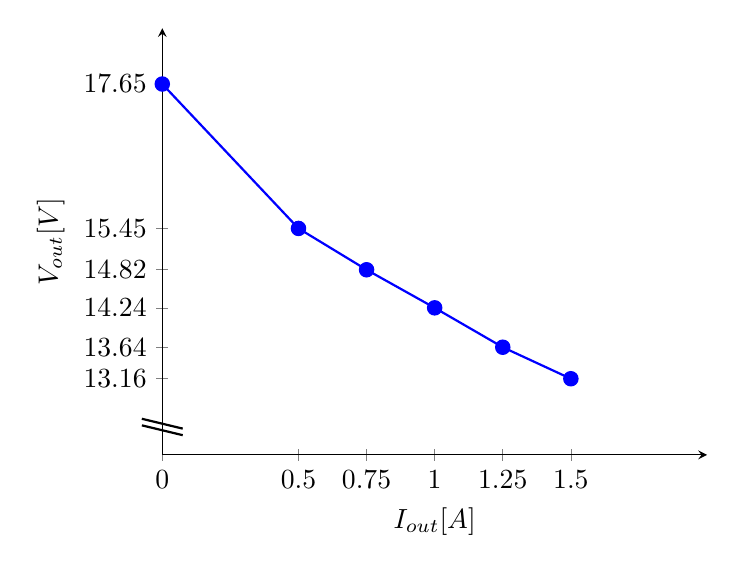
\begin{tikzpicture}
              \begin{axis}[
                axis lines = left,
                xlabel = {$I_{out}[A]$},
                ylabel = {$V_{out}[V]$},
                width=8.5cm,
                height=7cm,
                ymin=12, ymax=18.5,
                xmin=0, xmax=2,
                ytick={13.16,13.64,14.24,14.82,15.45,17.65},
                xtick={0,0.5,0.75,1,1.25,1.5},
                clip=false, % necesario para dibujar fuera del área del gráfico
              ]
                % Puntos conectados por líneas
                \addplot[
                  color=blue,
                  mark=*,
                  only marks,
                  mark options={scale=1.3}
                ]
                coordinates {
                  (0,17.65)(0.5,15.45) (0.75,14.82) (1.00,14.24) (1.25,13.64) (1.5,13.16)
                };
                
                \addplot[
                  color=blue,
                  thick
                ]
                coordinates {
                  (0,17.65)(0.5,15.45) (0.75,14.82) (1.00,14.24) (1.25,13.64) (1.5,13.16)
                };
                \draw[thick]
                  (axis cs:0.075,12.3) -- ++(-0.15,12.15);
                \draw[thick]
                  (axis cs:0.075,12.4) -- ++(-0.15,12.15);
              \end{axis}
            \end{tikzpicture}
          \end{minipage}%
          \caption{Tensión de salida de la fuente $V_{out}$ (punto bajo) en función de la corriente $I_{out}$ sobre una
                   carga variable}
          \label{fig:curva_salida_bajo}
        \end{figure}

        \subsubsection{Resistencia interna}
        
        Para calcular la resistencia interna se considera:

        \begin{equation*}
            R_{int} = \frac{V_{vacio} - V_{carga}}{I_{max}}= \frac{17.65V - 13.16V}{1.5A} = 2.99\Omega
        \end{equation*}

        \subsubsection{Regulación de voltaje}

        Por otro lado, se puede determinar el desempeño de la fuente para mantener la tensión constante frente a
        condiciones sin carga y con carga máxima mediante el siguiente cálculo:

        \begin{equation*}
            RV = \frac{V_{vacio} -V_{carga}}{V_{carga}} \times 100\% = \frac{17.65V-13.16V}{13.16V} \times 100\% = 34.1185\%
        \end{equation*}

        \subsubsection{Factor de ripple}
        
        Finalmente, el factor de ripple, que es un indicador de la efectividad del filtro se define como:

        \begin{equation*}
            FR = \frac{V_{eficaz-ripple}}{V_{carga}} \times 100\%
        \end{equation*}

        El $V_{eficaz-ripple}$ es la tensión medida con el multimétro establecido en escala de tensión alterna.
        Para ello, nos aseguramos de que el multimétro mida valor verdadero eficaz (true RMS) para realizar una
        medición más acertada. Considerando entonces el valor de $V_{eficaz-ripple}$ medido:

        \begin{equation*}
            FR = \frac{0.873V}{13.16V} \times 100\% = 6.6337\%
        \end{equation*}

        Además del uso del multimétro, nos pareció interesante observar la forma de onda de la tensión de salida de la
        fuente con el osciloscopio. De esta manera también pudimos observar el ripple calculado.
        \begin{figure}[!h]
          \centering
          \includegraphics[width=0.8\textwidth]{pictures/ripple_fuente-nreg.jpeg}
          \caption{Tensión de salida y observación del ripple de la fuente no regulada.}
        \end{figure}

        \subsection{Mediciones y cálculos: punto alto}
            Se procede de la misma manera que en el punto bajo, pero esta vez utilizando los dos bobinados del
            transformador:

        \begin{figure}[!h]
          % Minipage para la tabla
          \begin{minipage}{0.35\textwidth}
            \centering
            \begin{tabular}{|c|c|}
              \hline
              $I_{out}$ [A] & $V_{out}$ [V] \\
              \hline
              0.00 & 36.75 \\
              0.50 & 31.51 \\
              0.75 & 30.37\\
              1.00 & 28.92 \\
              1.25 & 27.76 \\
              1.50 & 26.62 \\
              \hline
            \end{tabular}
          \end{minipage}
          \begin{minipage}{0.35\textwidth}
            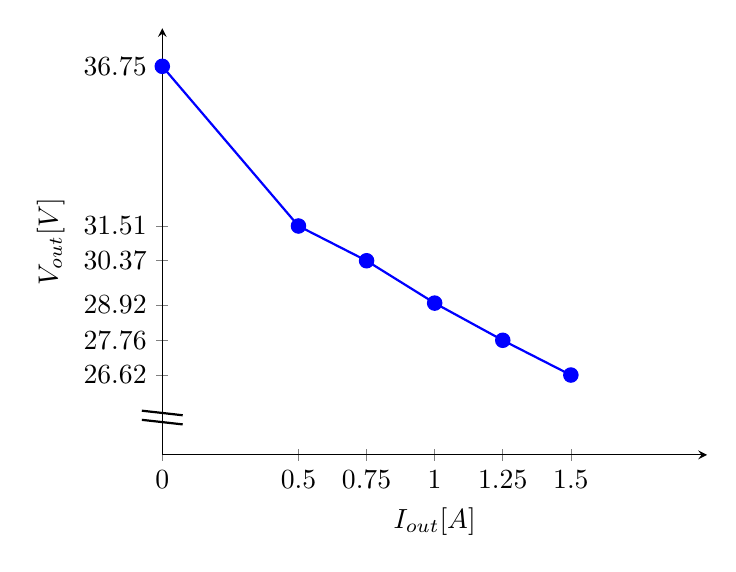
\begin{tikzpicture}
              \begin{axis}[
                axis lines = left,
                xlabel = {$I_{out}[A]$},
                ylabel = {$V_{out}[V]$},
                width=8.5cm,
                height=7cm,
                ymin=24, ymax=38,
                xmin=0, xmax=2,
                ytick={26.62,27.76,28.92,30.37,31.51,36.75},
                xtick={0,0.5,0.75,1,1.25,1.5},
                clip=false, % necesario para dibujar fuera del área del gráfico
              ]
                % Puntos conectados por líneas
                \addplot[
                  color=blue,
                  mark=*,
                  only marks,
                  mark options={scale=1.3}
                ]
                coordinates {
                  (0,36.75)(0.5,31.51) (0.75,30.37) (1.00,28.98) (1.25,27.76) (1.5,26.62)
                };
                
                \addplot[
                  color=blue,
                  thick
                ]
                coordinates {
                  (0,36.75)(0.5,31.51) (0.75,30.37) (1.00,28.98) (1.25,27.76) (1.5,26.62)
                };
                \draw[thick]
                  (axis cs:0.075,25) -- ++(-0.15,24.15);
                \draw[thick]
                  (axis cs:0.075,25.3) -- ++(-0.15,24.15);
              \end{axis}
            \end{tikzpicture}
          \end{minipage}
          \caption{Tensión de salida de la fuente $V_{out}$ (punto alto) en función de la corriente $I_{out}$ sobre una
                   carga variable.}
          \label{fig:curva_salida_alto}
        \end{figure}

        \subsubsection{Resistencia interna}

        Se calcula nuevamente la resistencia interna, ya que al utilizar los dos bobinados del transformador, ésta
        debe ser algo mayor:

        \begin{equation*}
            R_{int} = \frac{V_{vacio} - V_{carga}}{I_{max}}= \frac{36.75V - 26.62V}{1.5A} = 6.7533\Omega
        \end{equation*}

        \subsubsection{Regulación de voltaje}

        El desempeño de la fuente en el punto alto para mantener la tensión constante en distintas condiciones (sin carga
        y con carga máxima) es:

        \begin{equation*}
            RV = \frac{V_{vacio} -V_{carga}}{V_{carga}} \times 100\% = \frac{36.75V-26.62V}{26.62V} \times 100\% = 38.0541\%
        \end{equation*}

        \subsubsection{Factor de ripple}

        El factor de ripple en este caso, con un $V_{eficaz-ripple}=0.812V$ medido es:

        \begin{equation*}
            FR = \frac{V_{eficaz-ripple}}{V_{carga}} \times 100\% = \frac{0.812V}{26.62V} \times 100\% = 3.0503\%
        \end{equation*}

    \section{Fuente regulada}
      \begin{wrapfigure}{r}{0.4\textwidth}
        \centering
        \includegraphics[width=.4\textwidth]{pictures/reg_pcb.jpg}
        \caption{Fuente regulada en la PCB.}
      \end{wrapfigure}

      Las pruebas de la fuente regulada se hacen ya con toda la placa poblada. Para estas pruebas se utilizo el
      transformador en punto alto y ademas se conecto la fuente que genera el potencial negativo. Esta segunda fuente
      cumple el proposito de agregarle un extra de potencial negativo a la referencia de ajuste del LM317. Como
      resultado, el rango efectivo de ajuste del LM317 es ahora de 0 a 30V, mientras que sin la fuente negativa,
      el rango es de 1.25 a 30V.

      Como el objetivo del regulador es el de mejorar la salida, las mediciones que se van a hacer, son para
      compararlas con las de la fuente no regulada. De esta forma podemos destacar las ventajas y desventajas del uso
      de un regulador como el LM317

      Con toda la placa armada, esta se colocó en el banco de pruebas provisto por la facultad para realizar las
      mediciones. Es importante destacar que, debido a la potencia que discipa el LM317, es estrictamente necesario
      colocar el mismo en un discipador con pasta termica o algun otro medio de transferencia termica. El motivo de
      esto se va a explicar mas adelante.

      \begin{figure}[!h]
        \centering
        \includegraphics[width=0.8\textwidth]{pictures/reg_banco-prueb.jpeg}
        \caption{Placa montada en el banco de pruebas.}
      \end{figure}

      \subsection{Medicion de Regulacion de Voltaje}
        Nuevamente, para las mediciones de la regulacion de voltaje, se toma una medicion del potencial en la salida de
        la fuente sin carga y con carga plena:
        \begin{figure}[!h]
          \centering
          \begin{minipage}{0.4\textwidth}
            \begin{align*}
              V_{vacio} &= 15.84V\\[6pt]
              V_{carga} &= 15.54V
            \end{align*}
          \end{minipage}
          \begin{minipage}{0.4\textwidth}
            \begin{align*}
              RV &= \frac{V_{vacio} - V_{carga}}{V_{carga}} \times 100\%\\[6pt]
              RV &= \frac{15.84V - 15.54V}{15.54V} \times 100\%\\[6pt]
              RV &= 1.9\%
            \end{align*}
          \end{minipage}
        \end{figure}

      \subsection{Medicion de Ripple}
        Para la medicion de ripple, utilizamos un osciloscopio debido a que el LM317 tiene una atencuacion de al
        rededor de 1000 veces el ripple de entrada y ademas de que tiene una muy alta frecuencia. Esto imposibilita el
        uso de un multimetro True-RMS y ademas implica que la medicion del ripple puede estar errada. Con el
        osciloscopio obtuvimos lo siguiente:
        \begin{figure}[H]
          \centering
          \includegraphics[width=0.8\textwidth]{pictures/reg_osc-ripp.jpg}
          \caption{Ripple de salida de la fuente regulada, 40mv/div.}
        \end{figure}

        Por lo tanto:
        \begin{figure}[!h]
          \centering
          \begin{minipage}{0.4\textwidth}
            \begin{align*}
              V_{pp-ripple} &= 80mV\\[6pt]
              V_{carga} &= 15.54V
            \end{align*}
          \end{minipage}
          \begin{minipage}{0.4\textwidth}
            \begin{align*}
              FR &= \frac{V_{ef-ripple}}{V_{carga}} \times 100\%\\[6pt]
              FR &= \frac{\frac{40mV}{\sqrt{2}}}{15.54V} \times 100\%\\[6pt]
              FR &= 0.18\%
            \end{align*}
          \end{minipage}
        \end{figure}

      \subsection{Prueba termica}
        \begin{wrapfigure}{r}{0.4\textwidth}
          \centering
          \includegraphics[width=.4\textwidth]{pictures/reg_discipador.jpeg}
          \caption{Solucion de discipacion del banco de pruebas.}
        \end{wrapfigure}
        El motivo de esta prueba es comprobar que la solucion de discipacion termica es adecuada para la aplicacion y
        las condiciones de trabajo del LM317. Dado que utilizamos el empaquetado TO-220, la potencia maxima que puede
        discipar el LM317 es de 15W. Ademas, en la hoja de datos se indica que la temperatura maxima de la union
        (\textit{Maximum Junction Tempeure}) es de 125°C. Si la solucion de discipacion termica que empleamos no
        es capaz de mantener utemperatura de juntura igual o menor a 125°C, con el uso, la fuente va a reducir la
        potencia de salida para preservar su propia integridad y bajar la temperatura de juntura.

        La prueba consiste en hacer que el LM317 este en las condiciones mas extremas de trabajo, siendo estas la
        discipacion de 15W constantemente. Sabiendo que la corriente maxima del LM317 es de 1.5A, se puede determinar
        que la caida de tension tiene que ser 10V para que caigan 15W.

        Debido a que no es posible medir la temperatura de la juntura del silicio con el sustrato, el fabricante
        provee una relacion de la temperatura en la carcasa con la temperatura de juntura. Por eso, se mide la
        temperatura de carcasa ($T_C$) y con la formula de temperatura de juntura podemos saber si estamos
        debajo del limite.

        \begin{figure}[!h]
          \centering
          \includegraphics[width=0.8\textwidth]{pictures/reg_prueb-term.jpeg}
          \caption{Prueba termica. A la izquierda esta la temperatura de carcasa, abajo a la derecha la corriente y
                   arriba a la derecha la caida de tension en el LM317}
        \end{figure}

        Por lo tanto:
        \begin{figure}[!h]
          \centering
          \begin{minipage}{0.4\textwidth}
            \begin{align*}
              T_C &= 52^\circ C\\[6pt]
              V_{LM317} &= 10.09V\\[6pt]
              I_L &= 1.511A
            \end{align*}
          \end{minipage}
          \begin{minipage}{0.4\textwidth}
            \begin{align*}
              T_J &= \Theta_{JC} \cdot P_D + T_C\\[6pt]
              T_J &= 5\frac{^\circ C}{W} \cdot (10.09V \cdot 1.511A) + 52^\circ C\\[6pt]
              T_J &= 5\frac{^\circ C}{W} \cdot 15.25W + 52^\circ C\\[6pt]
              T_J &= 128.25^\circ C
            \end{align*}
          \end{minipage}
        \end{figure}

        A pesar de que la temperatura de juntura calculada esta por encima de los 125°C, podemos considerar como que
        el regulador va a compensar una pequeña cantidad de la potencia de salida para regular su temperatura de
        juntura. Ademas, segun las mediciones esta excedido en potencia, por lo que puede ser que la temperatura de
        juntura real sea menor. Por lo tanto, la solucion de discipacion de temperatura es la adecuada.

  \chapter{Conclusiones}
    En este trabajo pudimos comprender en profundidad el funcionamiento de cada una de las etapas que componen una fuente
    de alimentación lineal regulada, desde la transformación y rectificación hasta el filtrado y la regulación final.

    También analizamos la importancia de incorporar un regulador de tensión, observando cómo mejora la estabilidad de la
    salida y comparando su comportamiento frente a una fuente sin regulación. Esto nos permitió visualizar de forma
    práctica las ventajas que aporta en cuanto a protección y confiabilidad.

    Sin embargo, también vimos que este tipo de fuentes tienen sus limitaciones: si se las exige demasiado, tienden a 
    disipar gran parte de la energía en forma de calor, lo que afecta su eficiencia. Por lo tanto, son una buena solución
    en aplicaciones de baja o media exigencia, pero no siempre resultan viables cuando se requiere alta potencia o eficiencia energética.

\end{document}




